\documentclass{report}

% TODO: clean unused packages
% import templates created by SeniorMars
% \input{letterfonts}
% \input{macros}
\input{preamble}

\title{A Comprehensive Review of Agricultural Parcel and Boundary Delineation from Remote Sensing Images: Recent Progress and Future Perspectives}
\author{Juepeng Zheng et al.}
\date{}

\usepackage[backend=biber, style=authoryear]{biblatex}  % citations
\addbibresource{references.bib}                         % references file
\usepackage[font=small, textfont=bf]{caption}           % dont enumerate image captions
\usepackage{csquotes}                                   % for styled quotes
\usepackage{float}
\usepackage{graphicx}                                   % to import images
\graphicspath{{./images/}}                              % images dir
\usepackage{parskip}                                    % start paras on new lines instead of with indents

\begin{document}

\maketitle
\tableofcontents

\chapter{Research Summary}

% preface
\begin{center}
  \small
  \textbf{Preface} \\
  \vspace{1em}
  This report provides a comprehensive summary and critical analysis of 
  \citetitle{zheng2025comprehensivereviewagriculturalparcel} by \citeauthor{zheng2025comprehensivereviewagriculturalparcel} 
  The following sections synthesize the 
  authors' framework, methodology, and key findings regarding Agricultural 
  Parcel and Boundary Delineation (APBD)
  \vspace{1em}
\end{center}

\section{Introduction}

\dfn{Agricultural Parcel and Boundary Delineation}{
  \textbf{Agricultural Parcels} represent the fundamental spatial units for agricultural activity.
  \newline

  \textbf{Agricultural Parcel and Boundary Delineation (APBD)} is an interdisciplinary application of computer
  algorithms for vision tasks where agricultural fields are disected into their component parcels, and 
  distinctly separated from their background (adjacent parcels, natural vegetation and other types of land).
}

Applications of APBD include:
\begin{itemize}
  \item sustainable agriculture planning and land-use monitoring
  \item crop mapping
  \item yield estimation
\end{itemize}

Foundation models such as Transformer architectures, the Segment Anything Model (SAM), and Vision-Language
Vision-Language Models (VLMs), leveraging massive datasets and self-supervised learning, offer strong
generalizaton ability, high adaptability, and improved performance accross diverse agricultural
scenarios when applied to high-resolution remote sensing imagery.

The authors conceptualize APBD as composing three hierarchical levels:
\begin{enumerate}
  \item Cropland Identification
  \item Boundary Delineation 
  \item Parcel Segmentation
\end{enumerate}

The paper seeks to synthesize the emerging trends in APBD research, presenting the historical
evolution, current status, and future directions. The authors identify remote sensing data 
as a critical driver of APBD research in the foreseeable future.

\section{Meta-analysis of Related Literature}

\subsection{Overall Trend}
\begin{figure}[H]
    \centering
    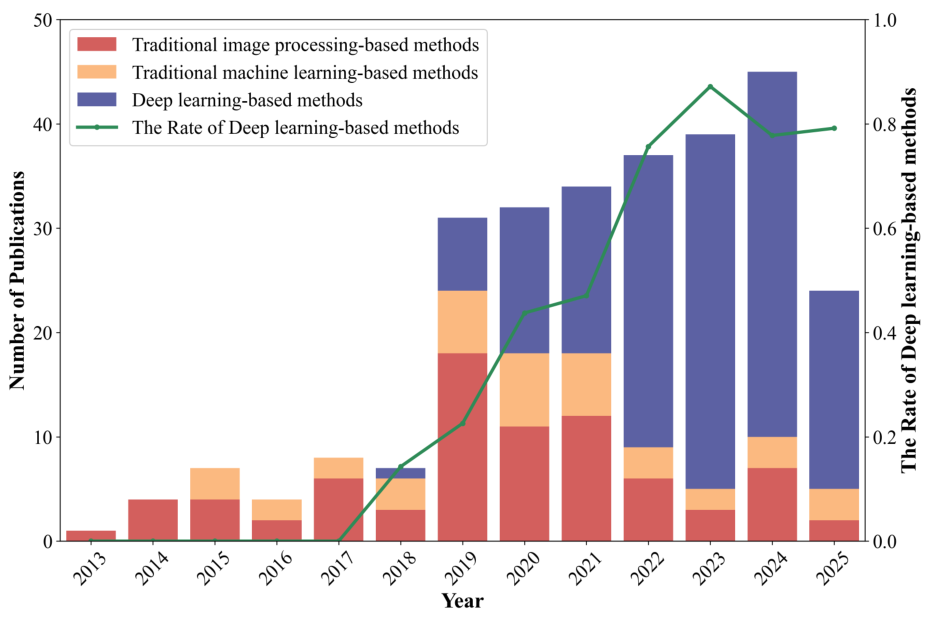
\includegraphics[width=0.7\textwidth]{fig-2}
    \caption*{Trends in APBD Methodologies (Figure 2)}
\end{figure}

\begin{itemize}
  \item \emph{\textquote{Since 2019, the number of APBD studies using Very High-Resolution (VHR) imagery has increased exponentially.}}
  \item Although VHR imagery enables high accuracy APBD, storage and processing costs prove to be a disadvantage. Large scale studies
    tend to use \textgreater 10 m spatial resolution to balance land variety and coverage, accuracy, and storage.
\end{itemize}

\chapter*{Acknowledgment}
\addcontentsline{toc}{chapter}{Acknowledgment}
This report is based entirely on the work of \citeauthor{zheng2025comprehensivereviewagriculturalparcel}. 
All concepts, findings, and frameworks presented herein are derived from 
their original research. No additional sources have been consulted for the 
core content of this summary.

\printbibliography[heading=bibintoc,title={References}]
\end{document}
